% this file is called up by thesis.tex
% content in this file will be fed into the main document
\chapter{Complementos}
% top level followed by section, subsection

\section{Lectura de listas}
\label{lectura.listas}


\newpage

\section{Gráficas de palabras nuevas entre dos idiomas}
\label{palabras.nuevas.apendice}

\begin{figure}[h!]
	\centering
	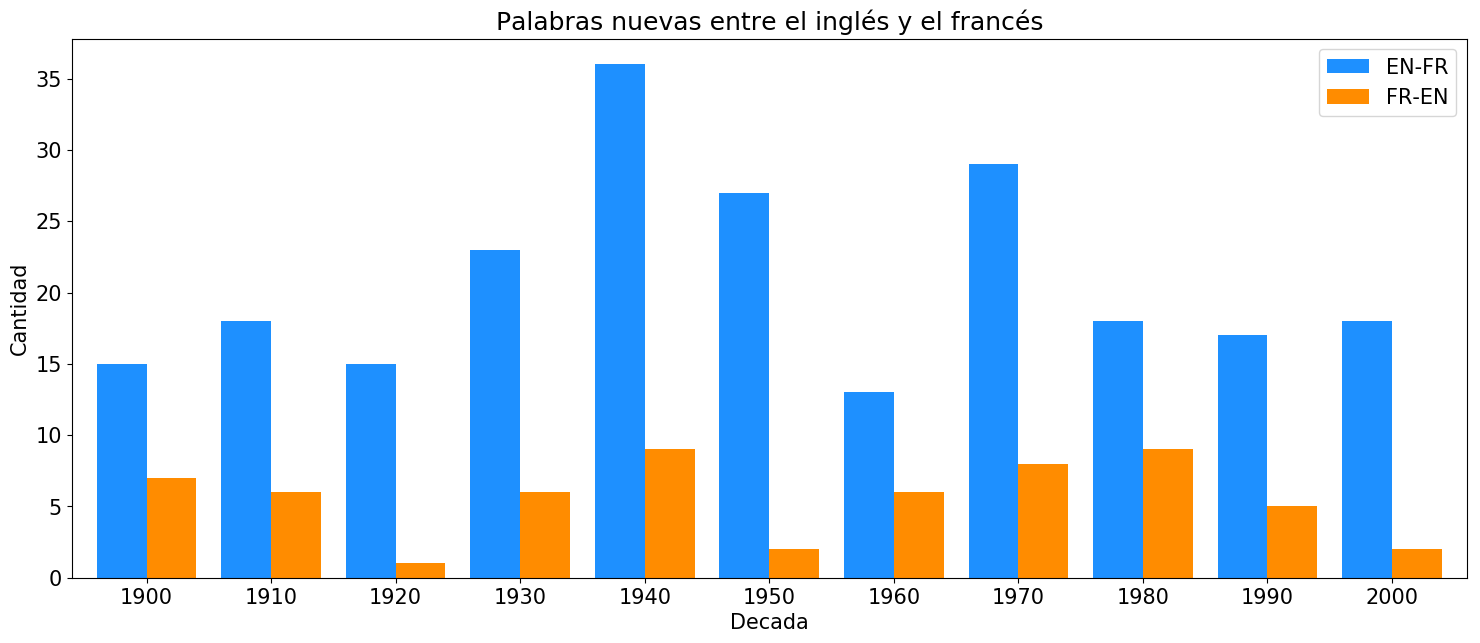
\includegraphics[scale=.38]{NC_1_S2_EN.png}
	\label{fig.NC_EF}
	\caption{Palabras nuevas entre el inglés y el francés}
\end{figure}

\begin{figure}[h!]
	\centering
	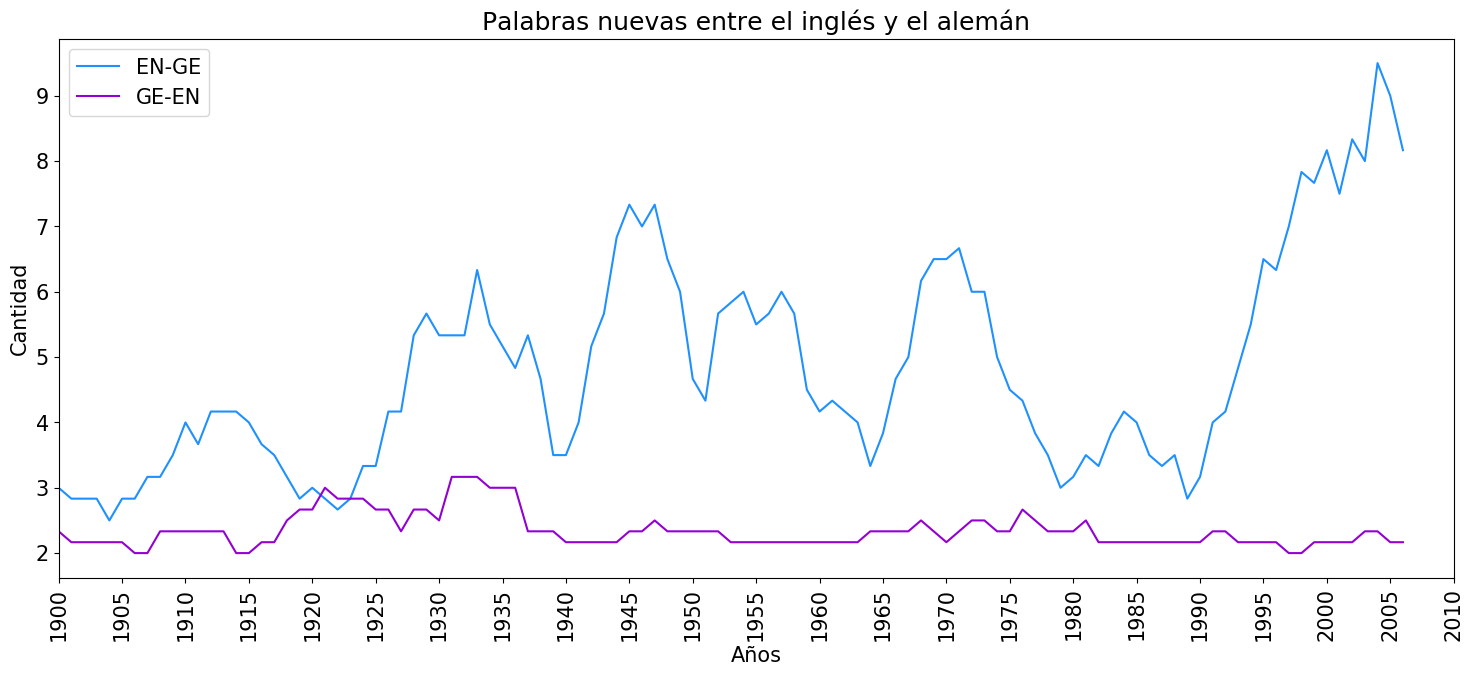
\includegraphics[scale=.38]{NC_2_S2_EN.png}
	\label{fig.NC_EG}
	\caption{Palabras nuevas entre el inglés y el alemán}
\end{figure}

\begin{figure}[h!]
	\centering
	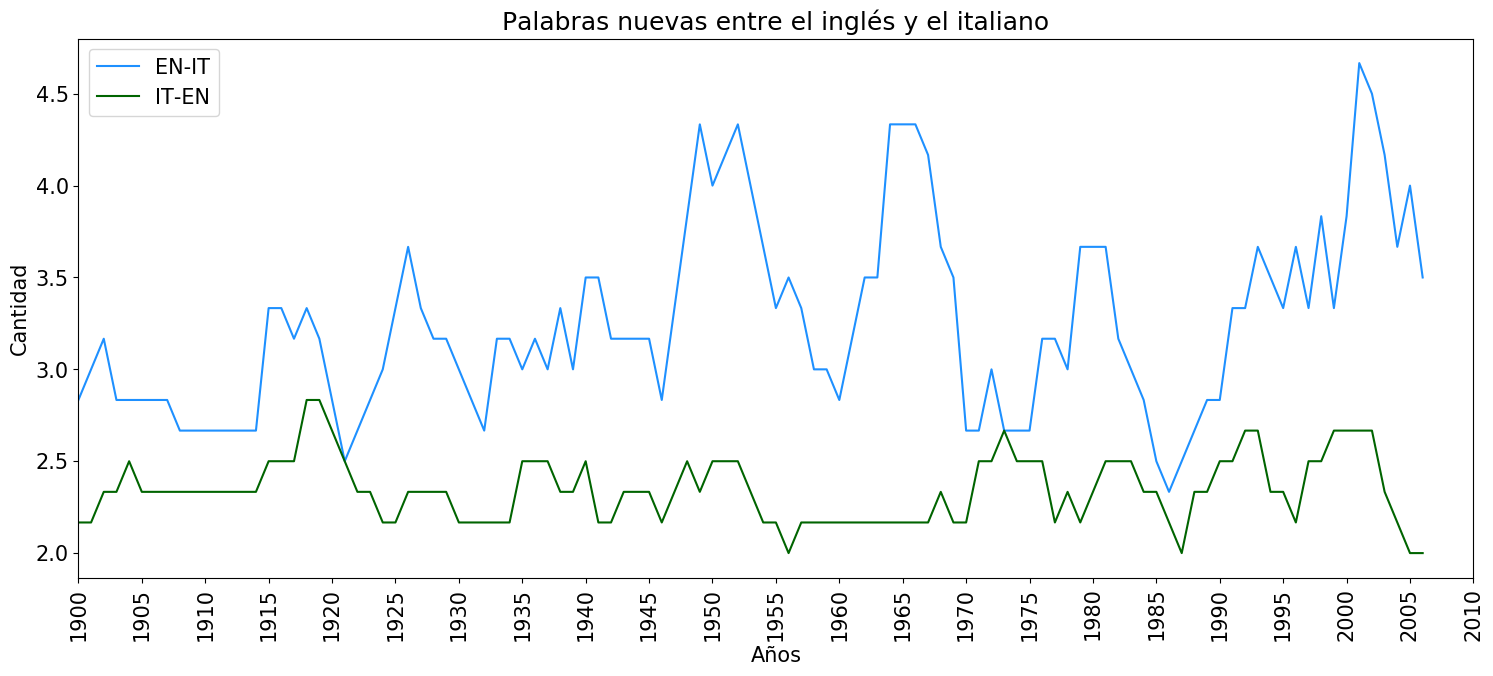
\includegraphics[scale=.38]{NC_3_S2_EN.png}
	\label{fig.NC_EI}
	\caption{Palabras nuevas entre el inglés y el italiano}
\end{figure}


\begin{figure}[h!]
	\centering
	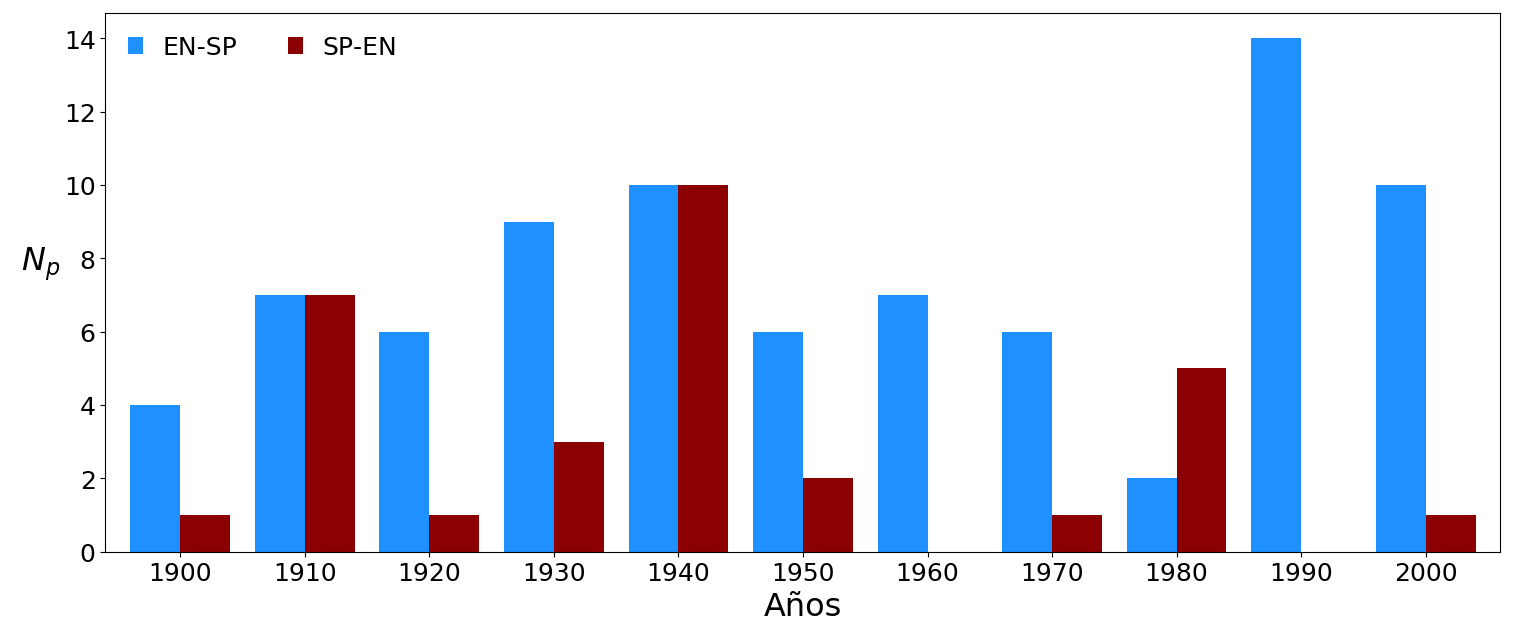
\includegraphics[scale=.38]{NC_4_S2_EN.png}
	\label{fig.NC_ES}
	\caption{Palabras nuevas entre el inglés y el español}
\end{figure}

\begin{figure}[h!]
	\centering
	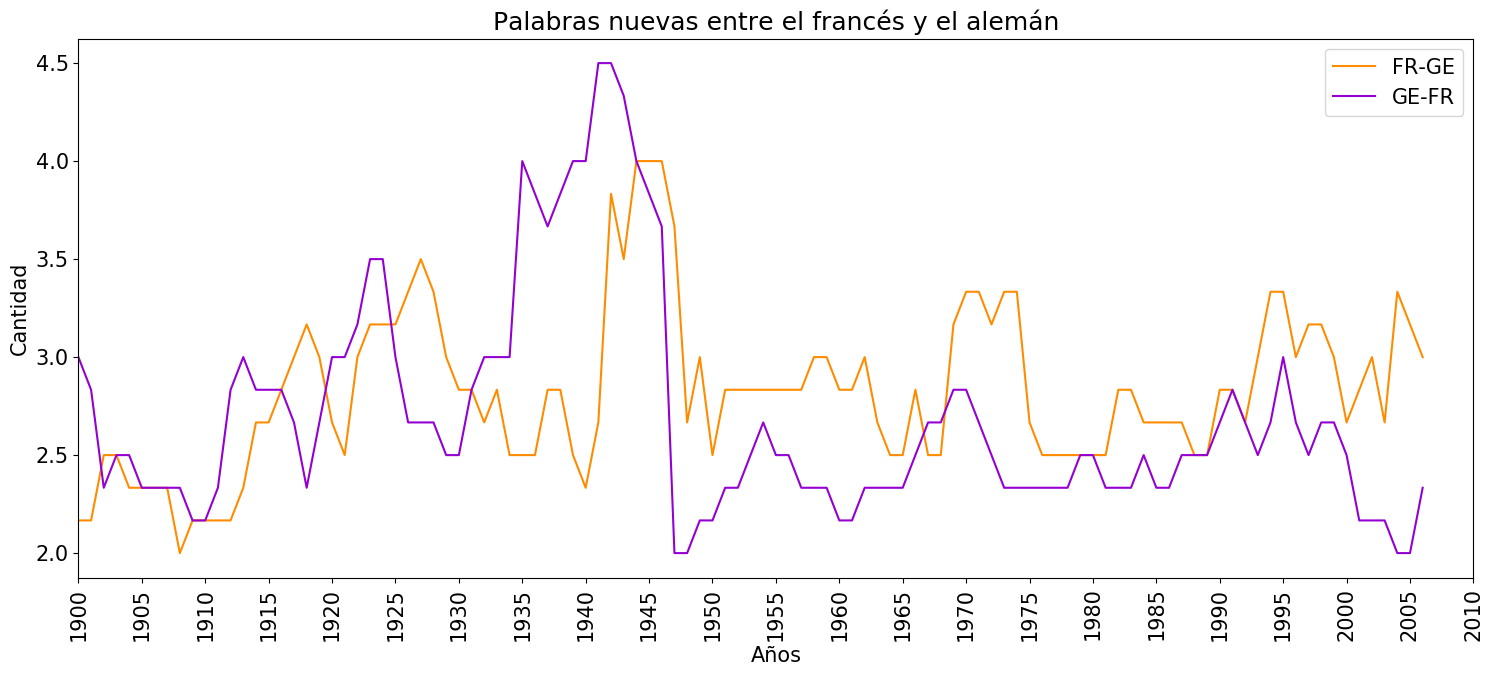
\includegraphics[scale=.38]{NC_2_S2_FR.png}
	\label{fig.NC_FG}
	\caption{Palabras nuevas entre el francés y el alemán}
\end{figure}


\begin{figure}[h!]
	\centering
	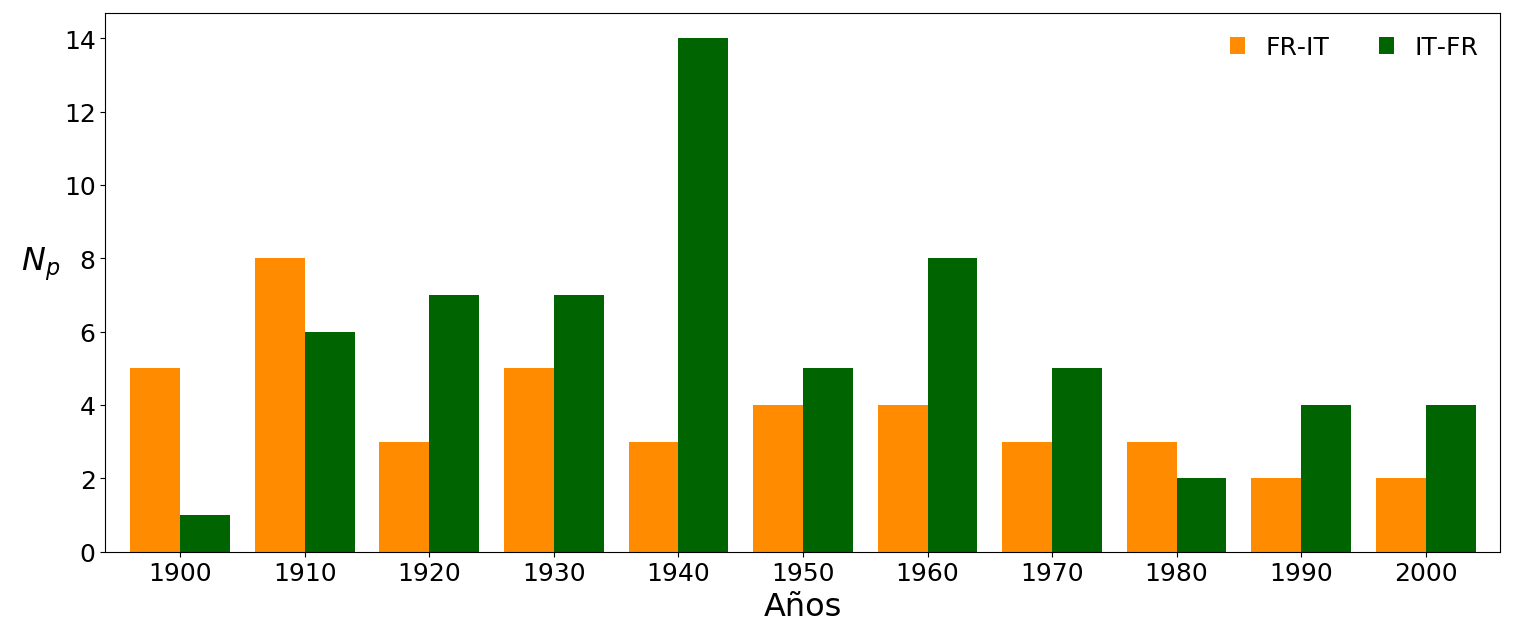
\includegraphics[scale=.38]{NC_3_S2_FR.png}
	\label{fig.NC_FI}
	\caption{Palabras nuevas entre el francés y el italiano}
\end{figure}

\begin{figure}[h!]
	\centering
	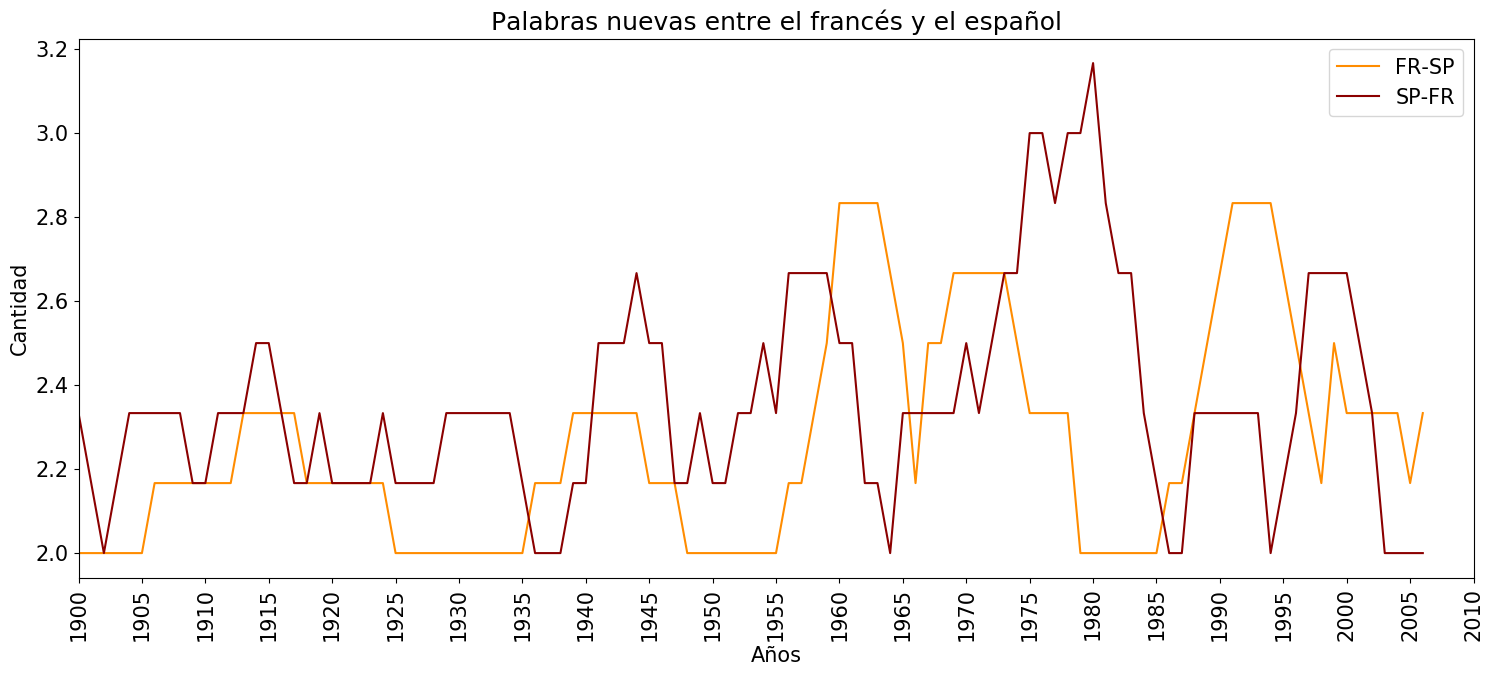
\includegraphics[scale=.38]{NC_4_S2_FR.png}
	\label{fig.NC_FS}
	\caption{Palabras nuevas entre el francés y el español}
\end{figure}

\begin{figure}[h!]
	\centering
	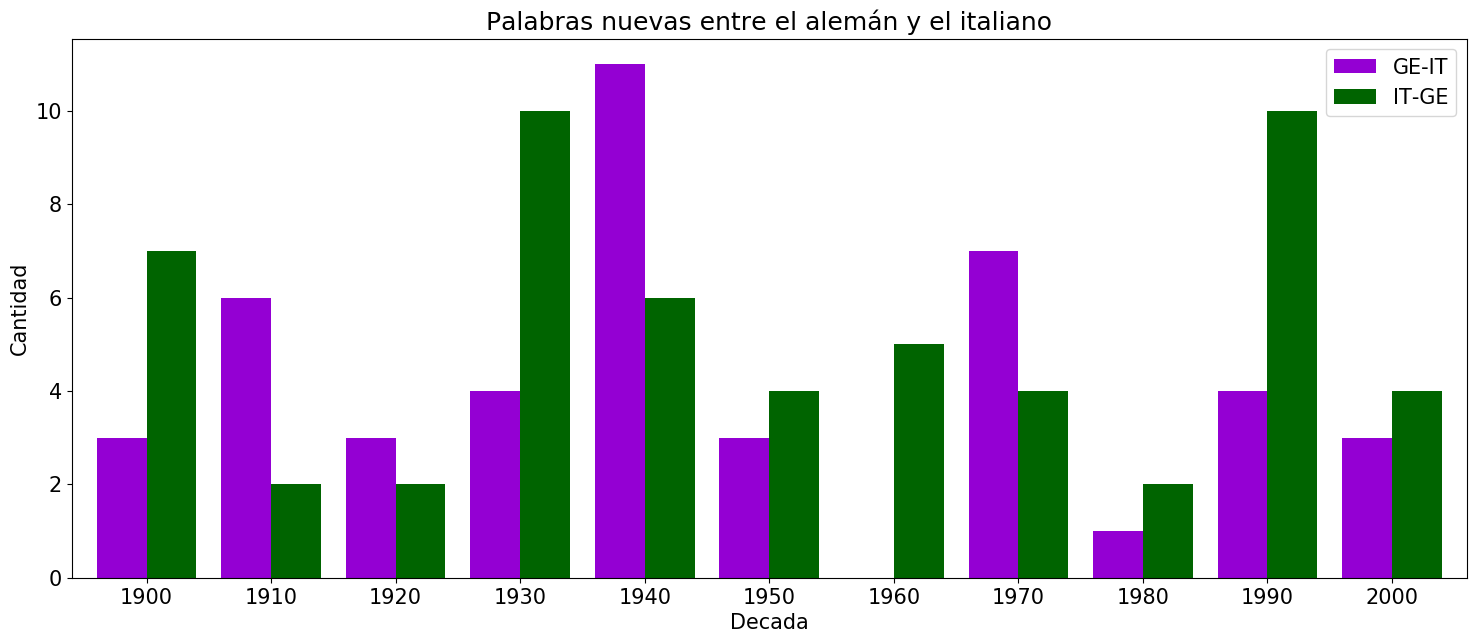
\includegraphics[scale=.38]{NC_3_S2_GE.png}
	\label{fig.NC_GI}
	\caption{Palabras nuevas entre el alemán y el italiano}
\end{figure}

\begin{figure}[h!]
	\centering
	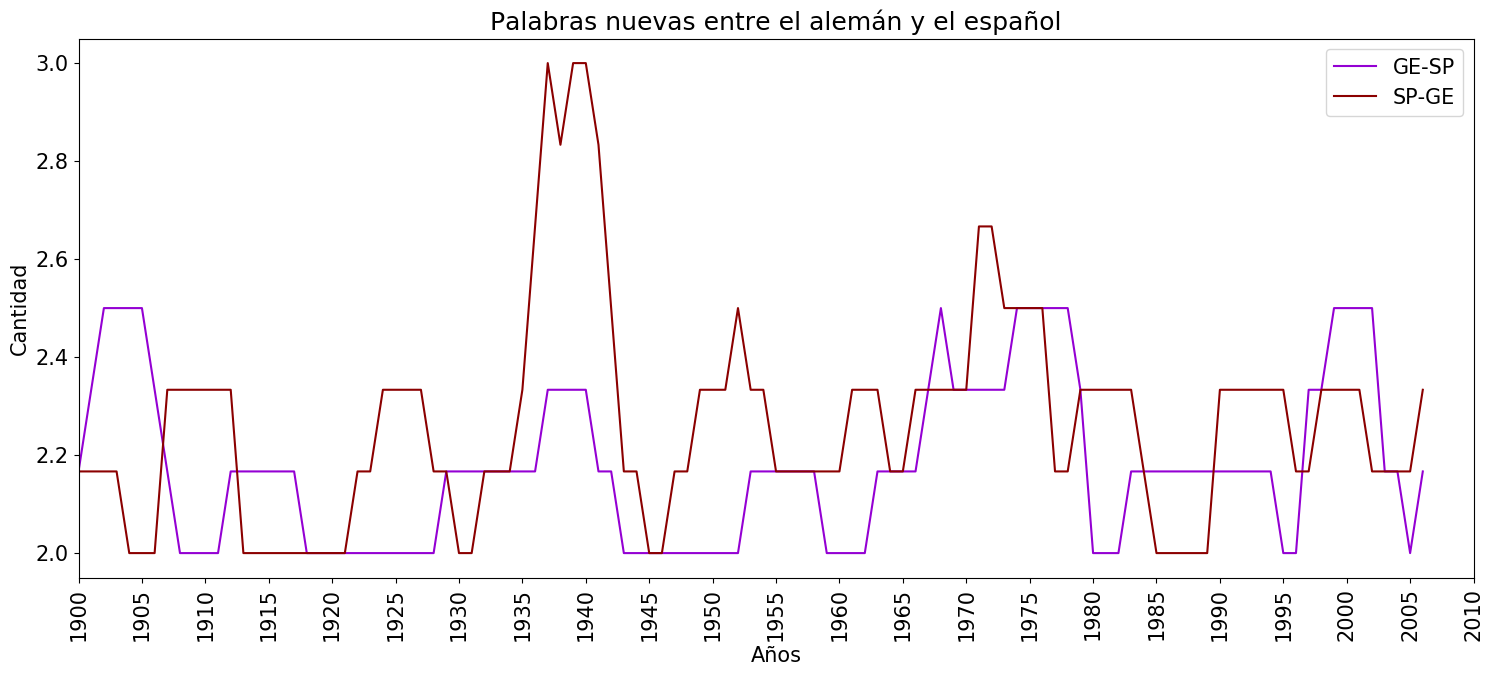
\includegraphics[scale=.38]{NC_4_S2_GE.png}
	\label{fig.NC_GS}
	\caption{Palabras nuevas entre el alemán y el español}
\end{figure}

\begin{figure}[h!]
	\centering
	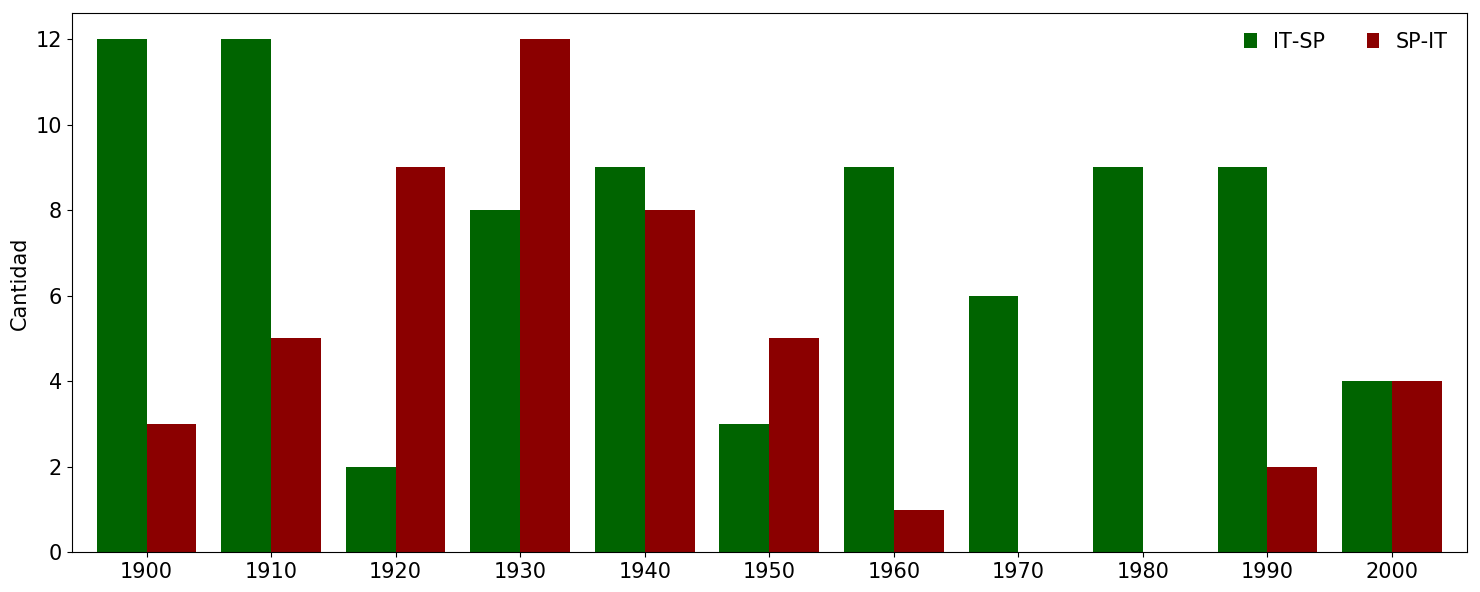
\includegraphics[scale=.38]{NC_4_S2_IT.png}
	\label{fig.NC_IS}
	\caption{Palabras nuevas entre el italiano y el español}
\end{figure}





\clearpage



\section{Gráficas de palabras acumuladas entre dos idiomas}
\label{palabras.acumuladas.apendice}

\begin{figure}[h!]
	\centering
	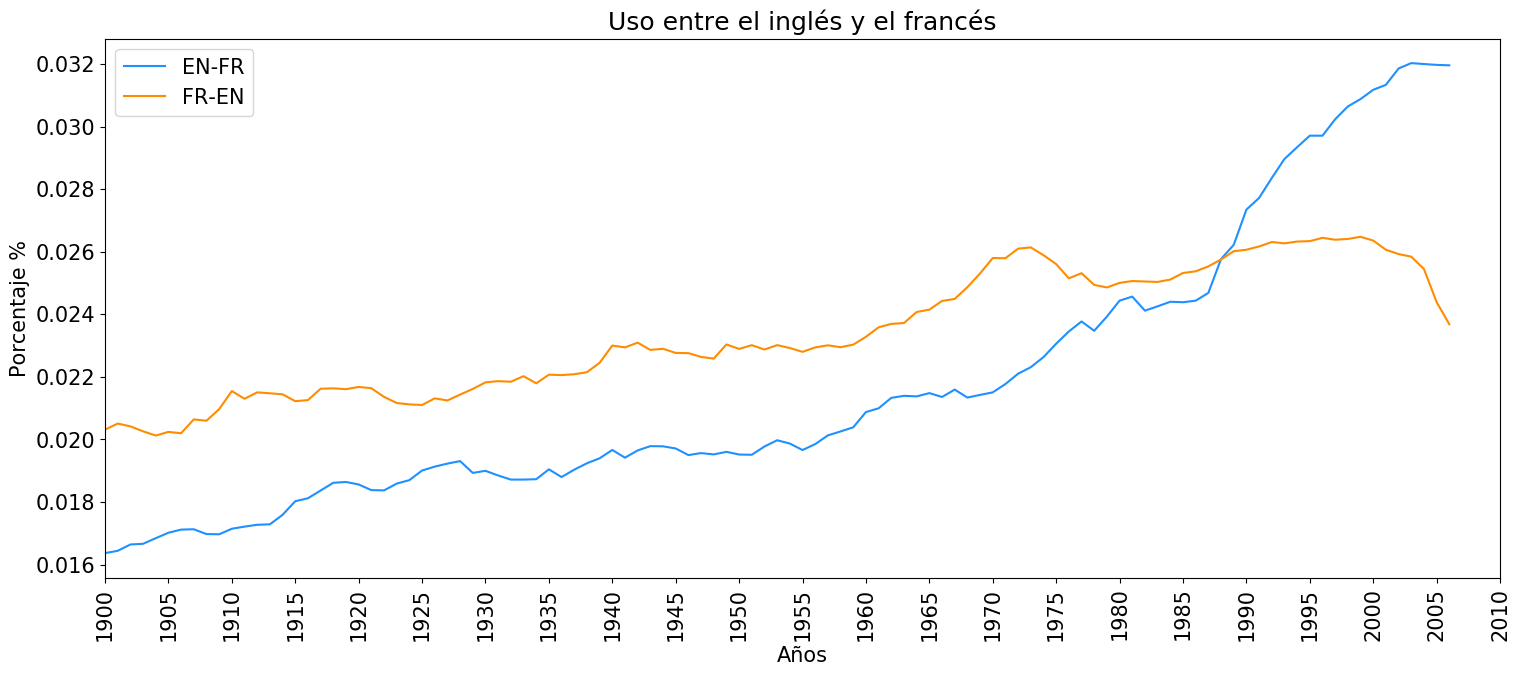
\includegraphics[scale=.38]{SF_1_S2_EN.png}
	\label{fig.SF_EF}
	\caption{Palabras acumuladas entre el inglés y el francés}
\end{figure}


\begin{figure}[h!]
	\centering
	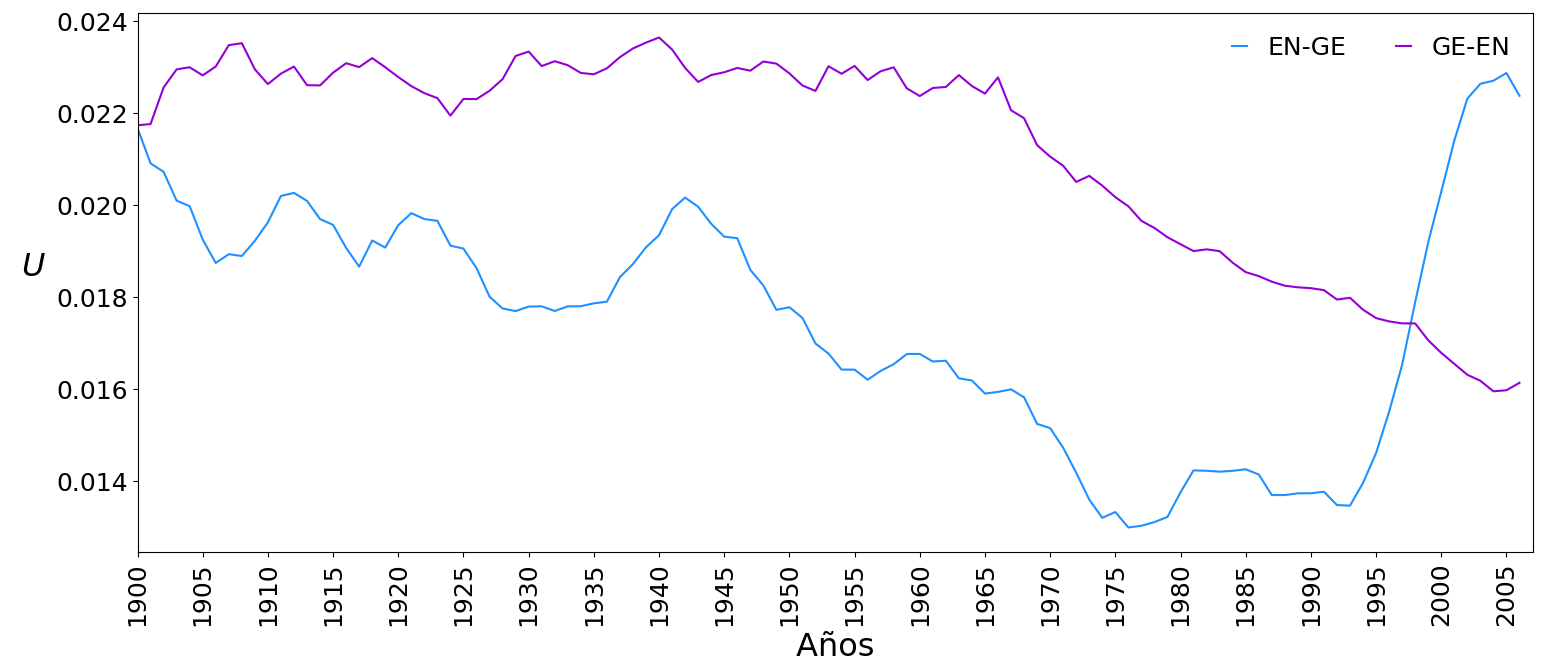
\includegraphics[scale=.38]{SF_2_S2_EN.png}
	\label{fig.SF_EG}
	\caption{Palabras acumuladas entre el inglés y el alemán}
\end{figure}


\begin{figure}[h!]
	\centering
	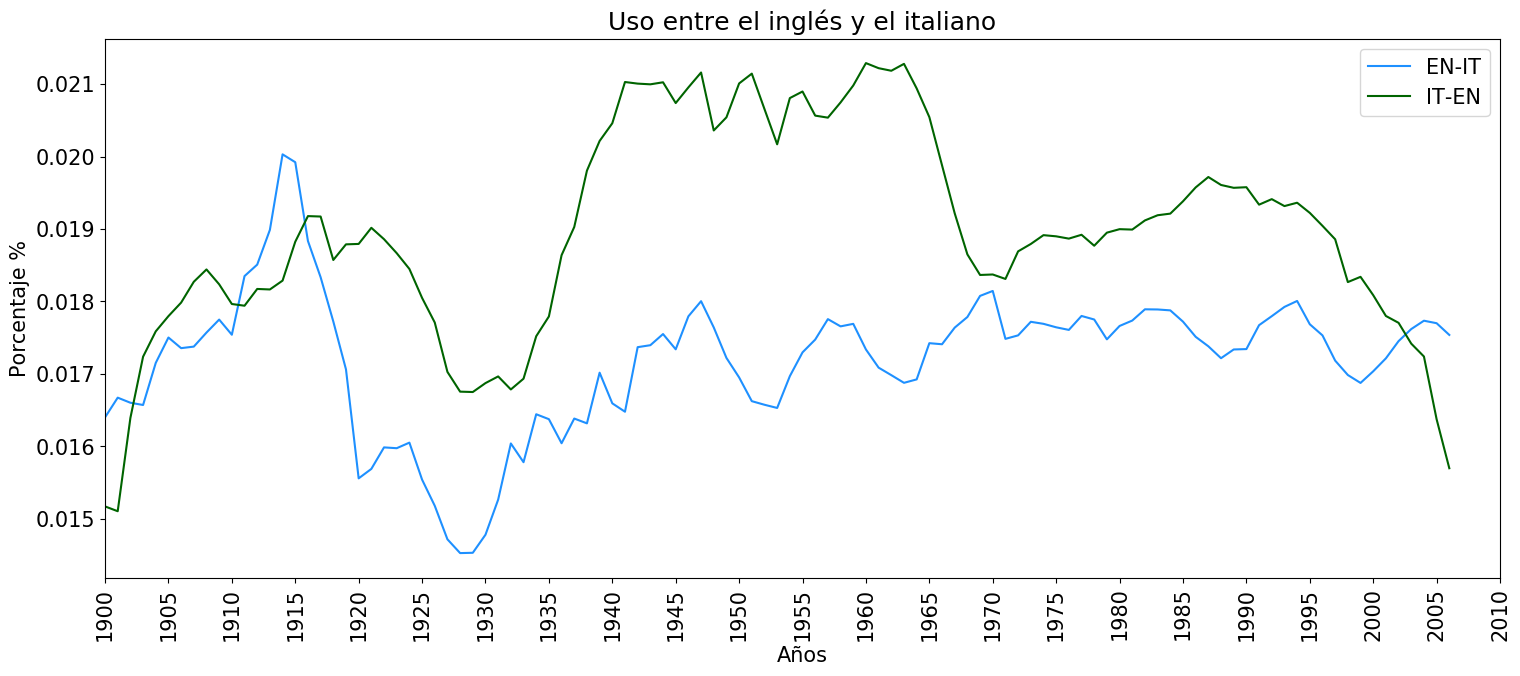
\includegraphics[scale=.38]{SF_3_S2_EN.png}
	\label{fig.SF_EI}
	\caption{Palabras acumuladas entre el inglés y el italiano}
\end{figure}

\begin{figure}[h!]
	\centering
	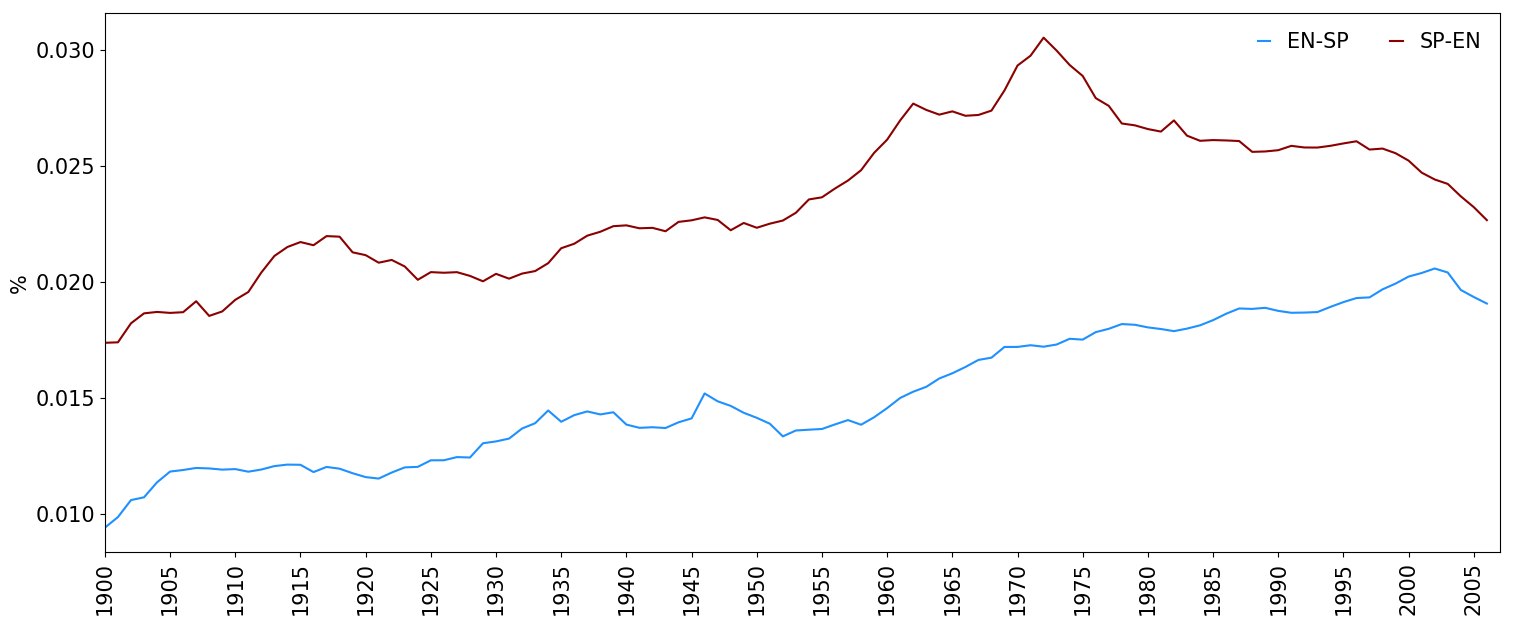
\includegraphics[scale=.38]{SF_4_S2_EN.png}
	\label{fig.SF_ES}
	\caption{Palabras acumuladas entre el inglés y el español}
\end{figure}

\begin{figure}[h!]
	\centering
	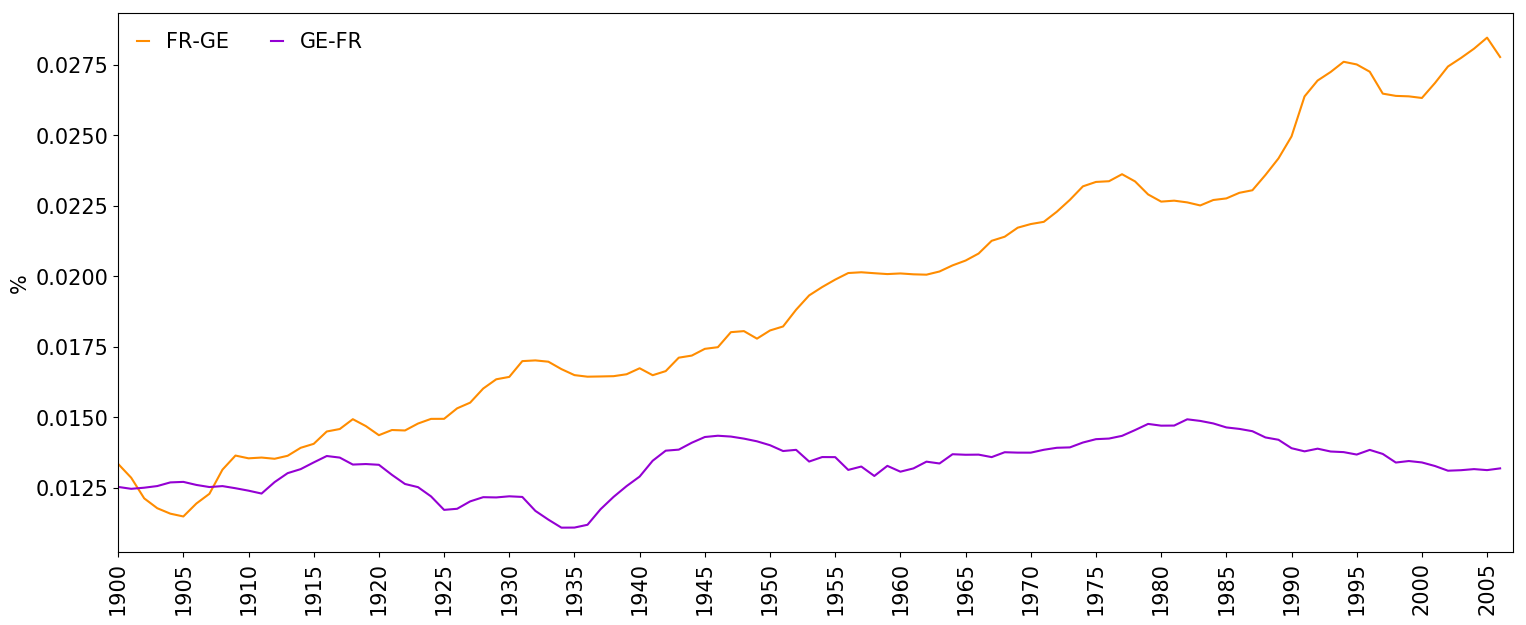
\includegraphics[scale=.38]{SF_2_S2_FR.png}
	\label{fig.SF_FG}
	\caption{Palabras acumuladas entre el francés y el alemán}
\end{figure}

\begin{figure}[h!]
	\centering
	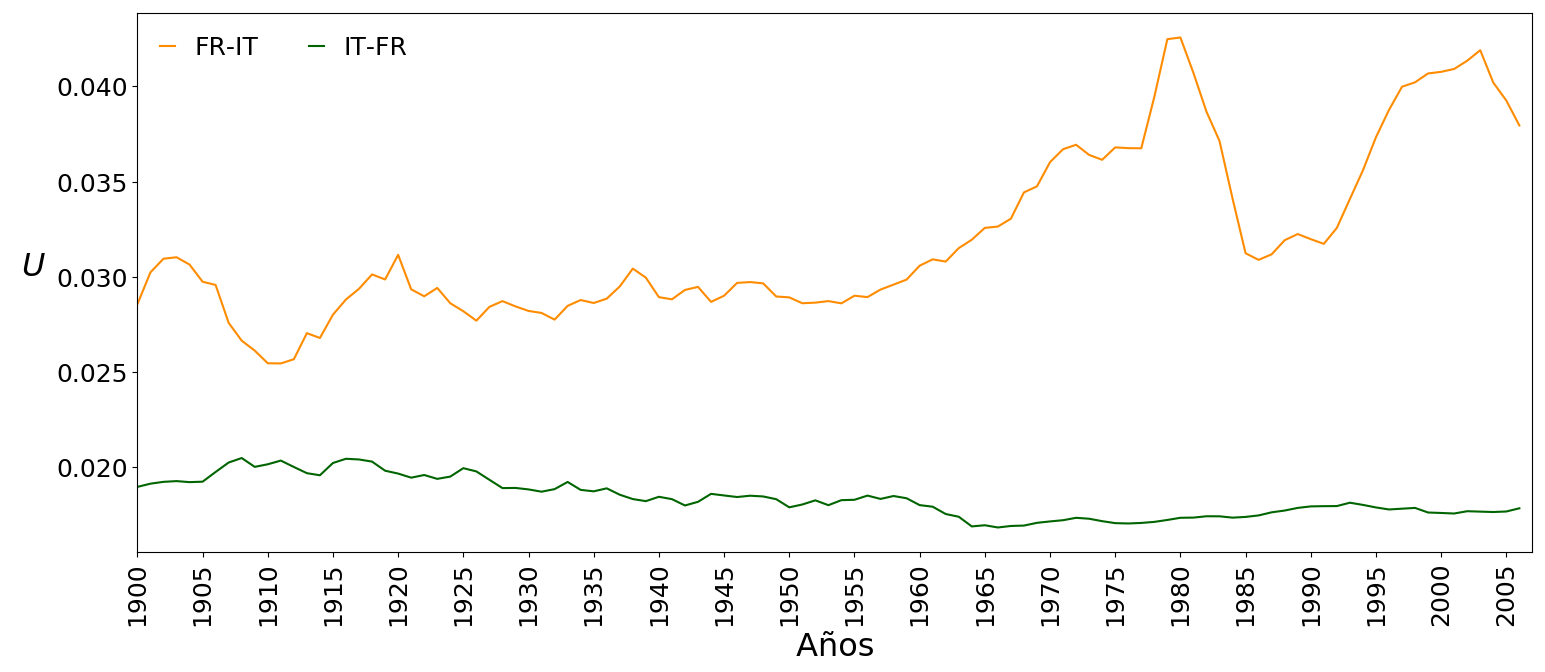
\includegraphics[scale=.38]{SF_3_S2_FR.png}
	\label{fig.SF_FI}
	\caption{Palabras acumuladas entre el francés y el italiano}
\end{figure}

\begin{figure}[h!]
	\centering
	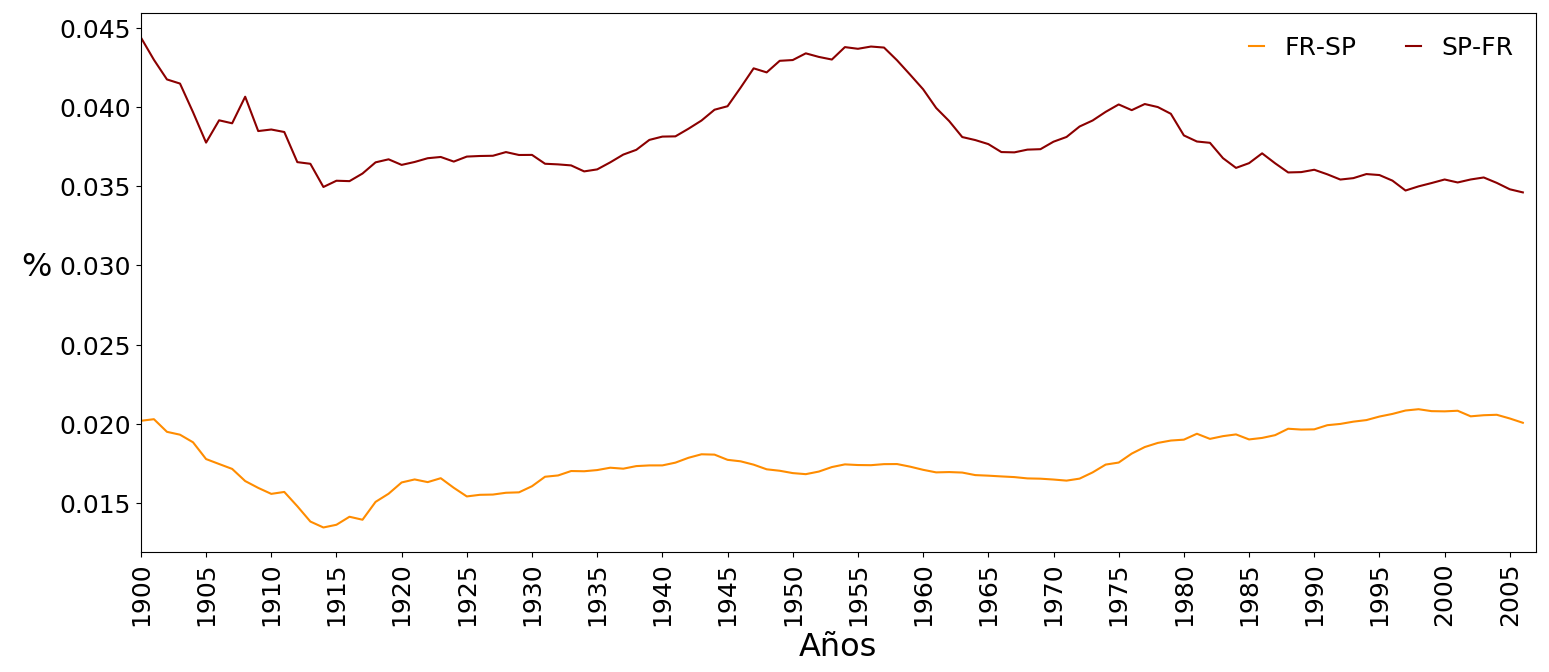
\includegraphics[scale=.38]{SF_4_S2_FR.png}
	\label{fig.SF_FS}
	\caption{Palabras acumuladas entre el francés y el español}
\end{figure}



\begin{figure}[h!]
	\centering
	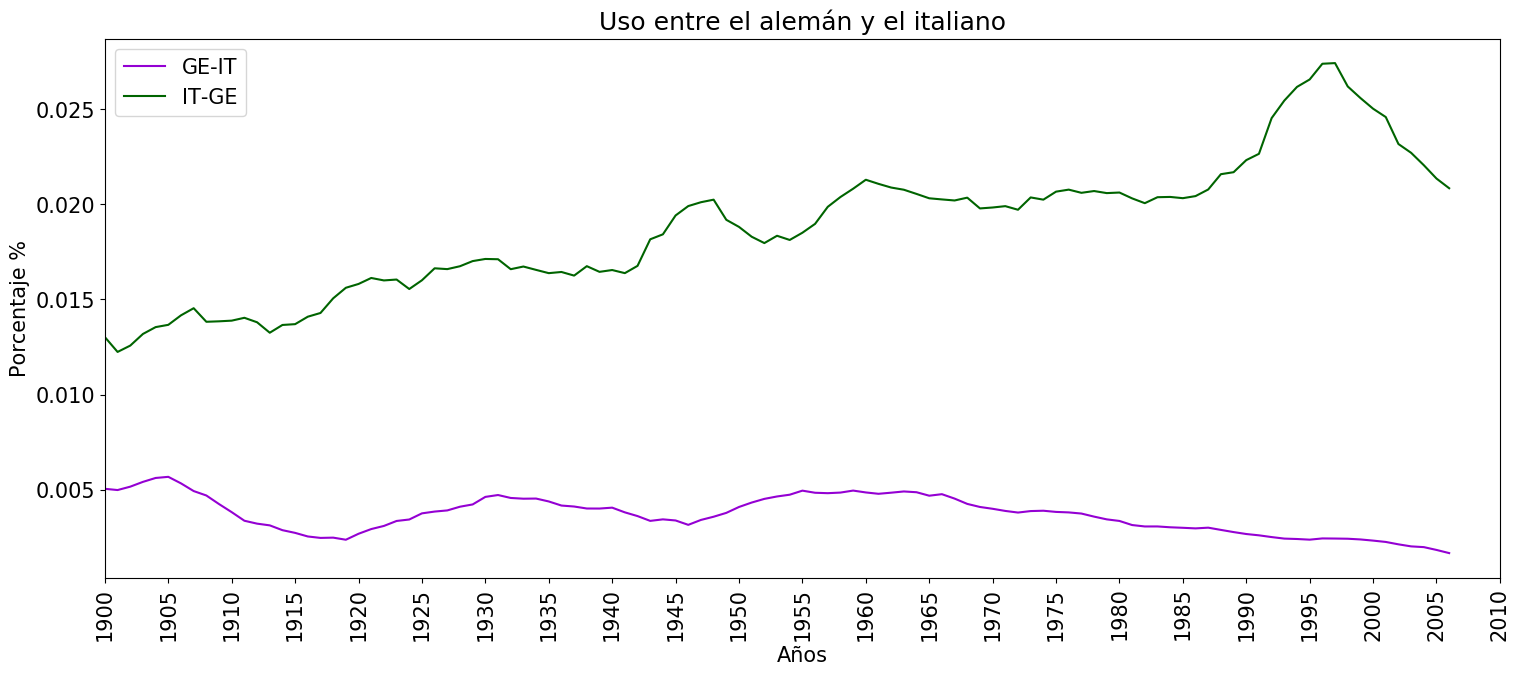
\includegraphics[scale=.38]{SF_3_S2_GE.png}
	\label{fig.SF_GI}
	\caption{Palabras acumuladas entre el alemán y el italiano}
\end{figure}


\begin{figure}[h!]
	\centering
	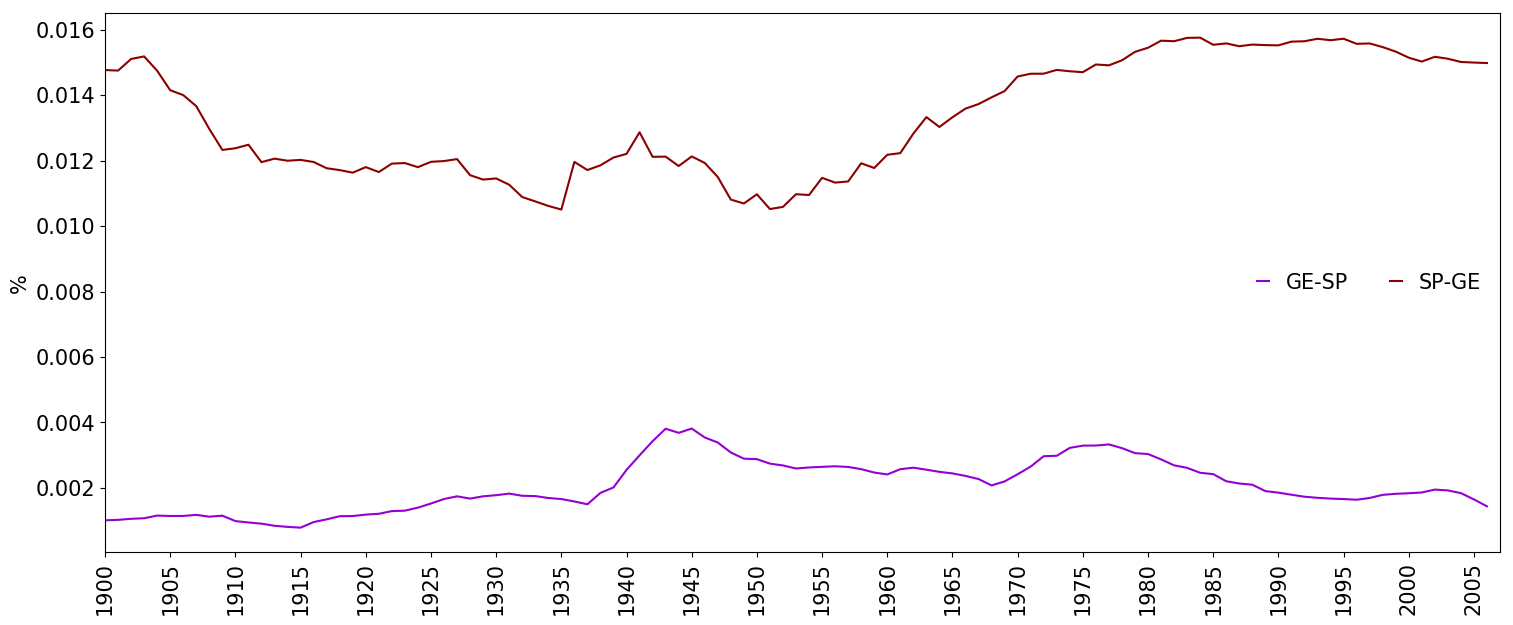
\includegraphics[scale=.38]{SF_4_S2_GE.png}
	\label{fig.SF_GS}
	\caption{Palabras acumuladas entre el alemán y el español}
\end{figure}


\begin{figure}[h!]
	\centering
	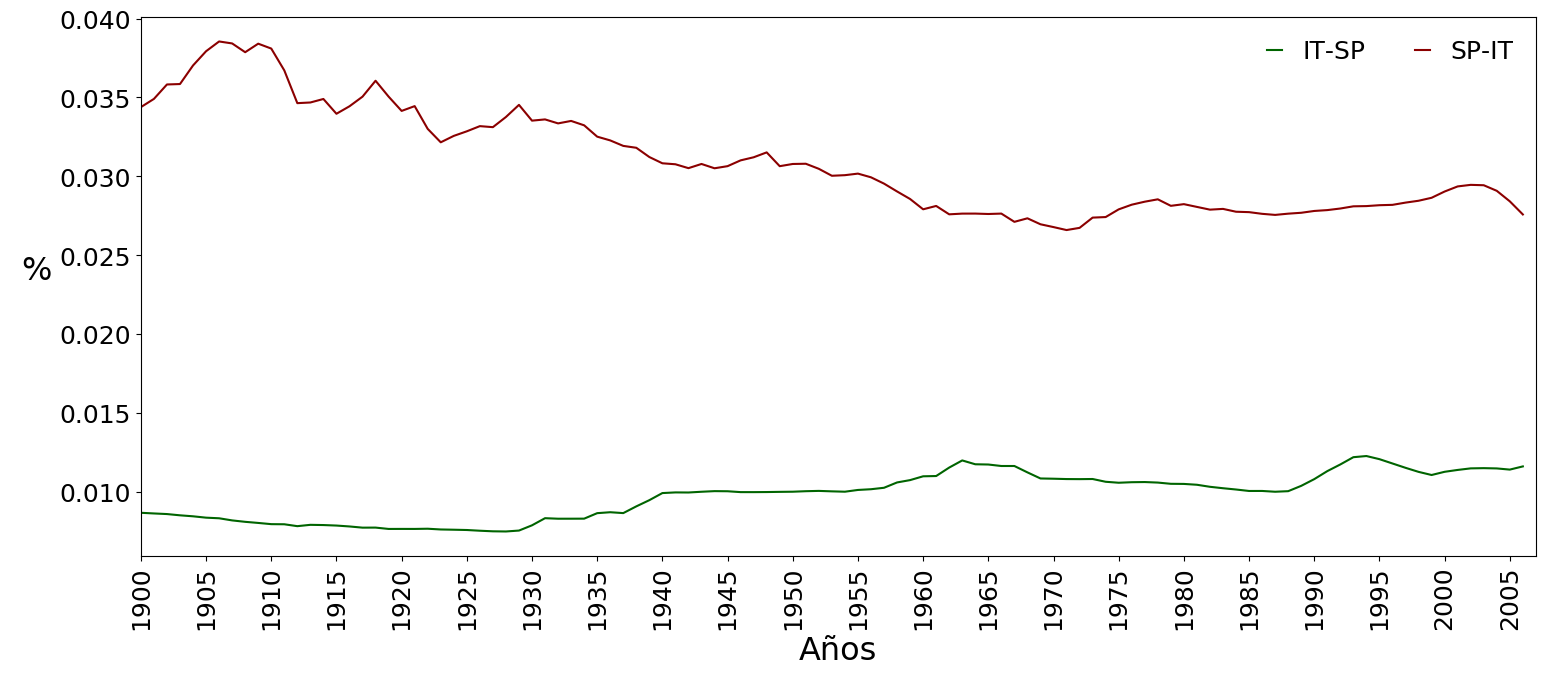
\includegraphics[scale=.38]{SF_4_S2_IT.png}
	\label{fig.SF_IS}
	\caption{Palabras acumuladas entre el italiano y el español}
\end{figure}
